\section{Zeichnungen}
\label{sec:anhang_a}
% Inhalt: Rad 2022-03-16, Ritzel 2022-06-23 und 2025-04-02 (30_references_and_examples/93_Zeichnungen).

Die Zeichnungen des Kunststoffrades (Ausgabedatum 28.02.2022) sowie des Stahlritzels (08.06.2022 und 02.04.2025) liegen als Einzelteilzeichnungen der Forschungsstelle vor und sind auf den folgenden drei Seiten wiedergegeben. Die daraus übernommenen Werte nennt \secref{sec:pruefverzahnung}.

% Seiten aus 30_references_and_examples/93_Zeichnungen (Kopien unter bilder/anhang, 2026-10-25); pdfpages lädt die Klasse.
% Maßstab 0,78 und 4 mm nach unten wie die Protokolle in A.7, damit der Zeichnungsrahmen unter der Kopfzeile bleibt (Nutzer, 2026-10-26).
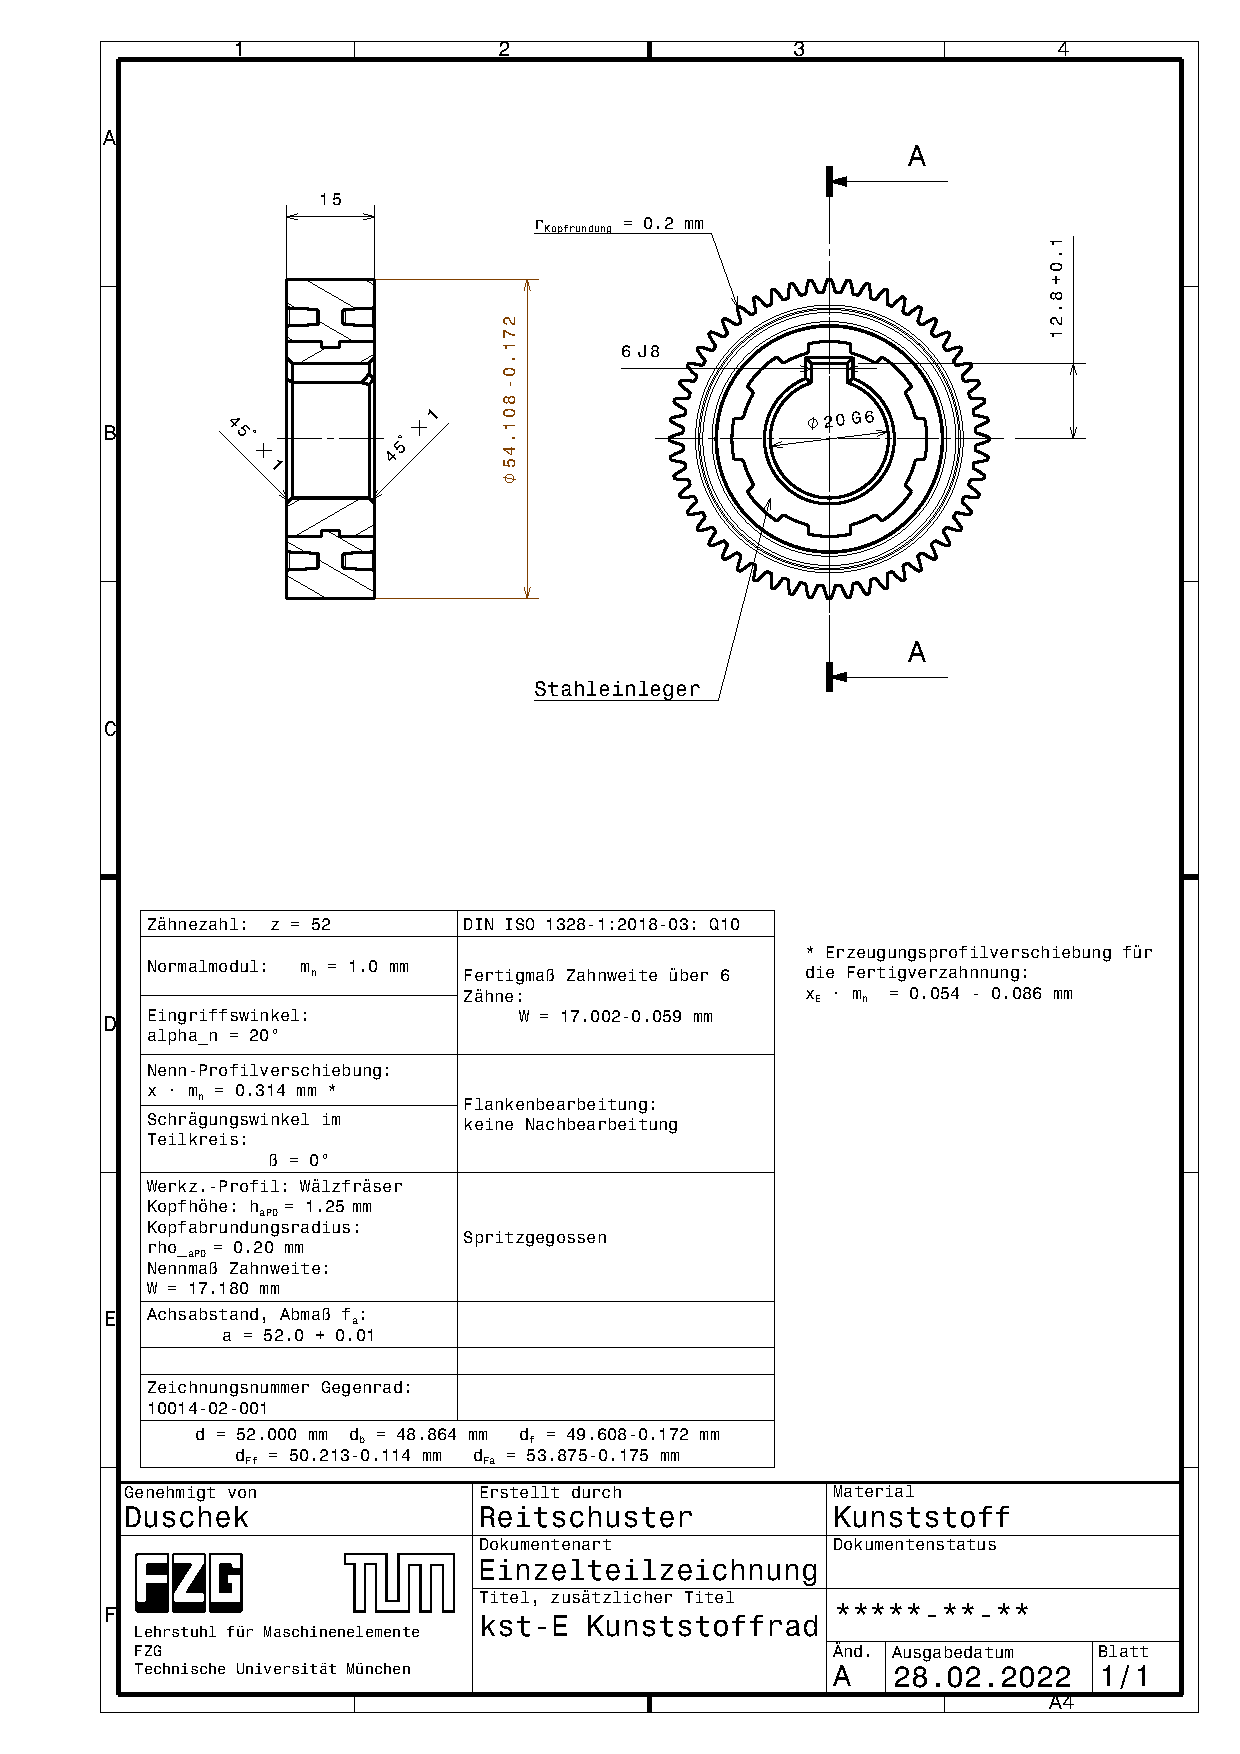
\includepdf[pages=1, scale=0.78, offset=0 -4mm, pagecommand={\thispagestyle{plain}}]{anhang/zeichnung_rad_2022.pdf}
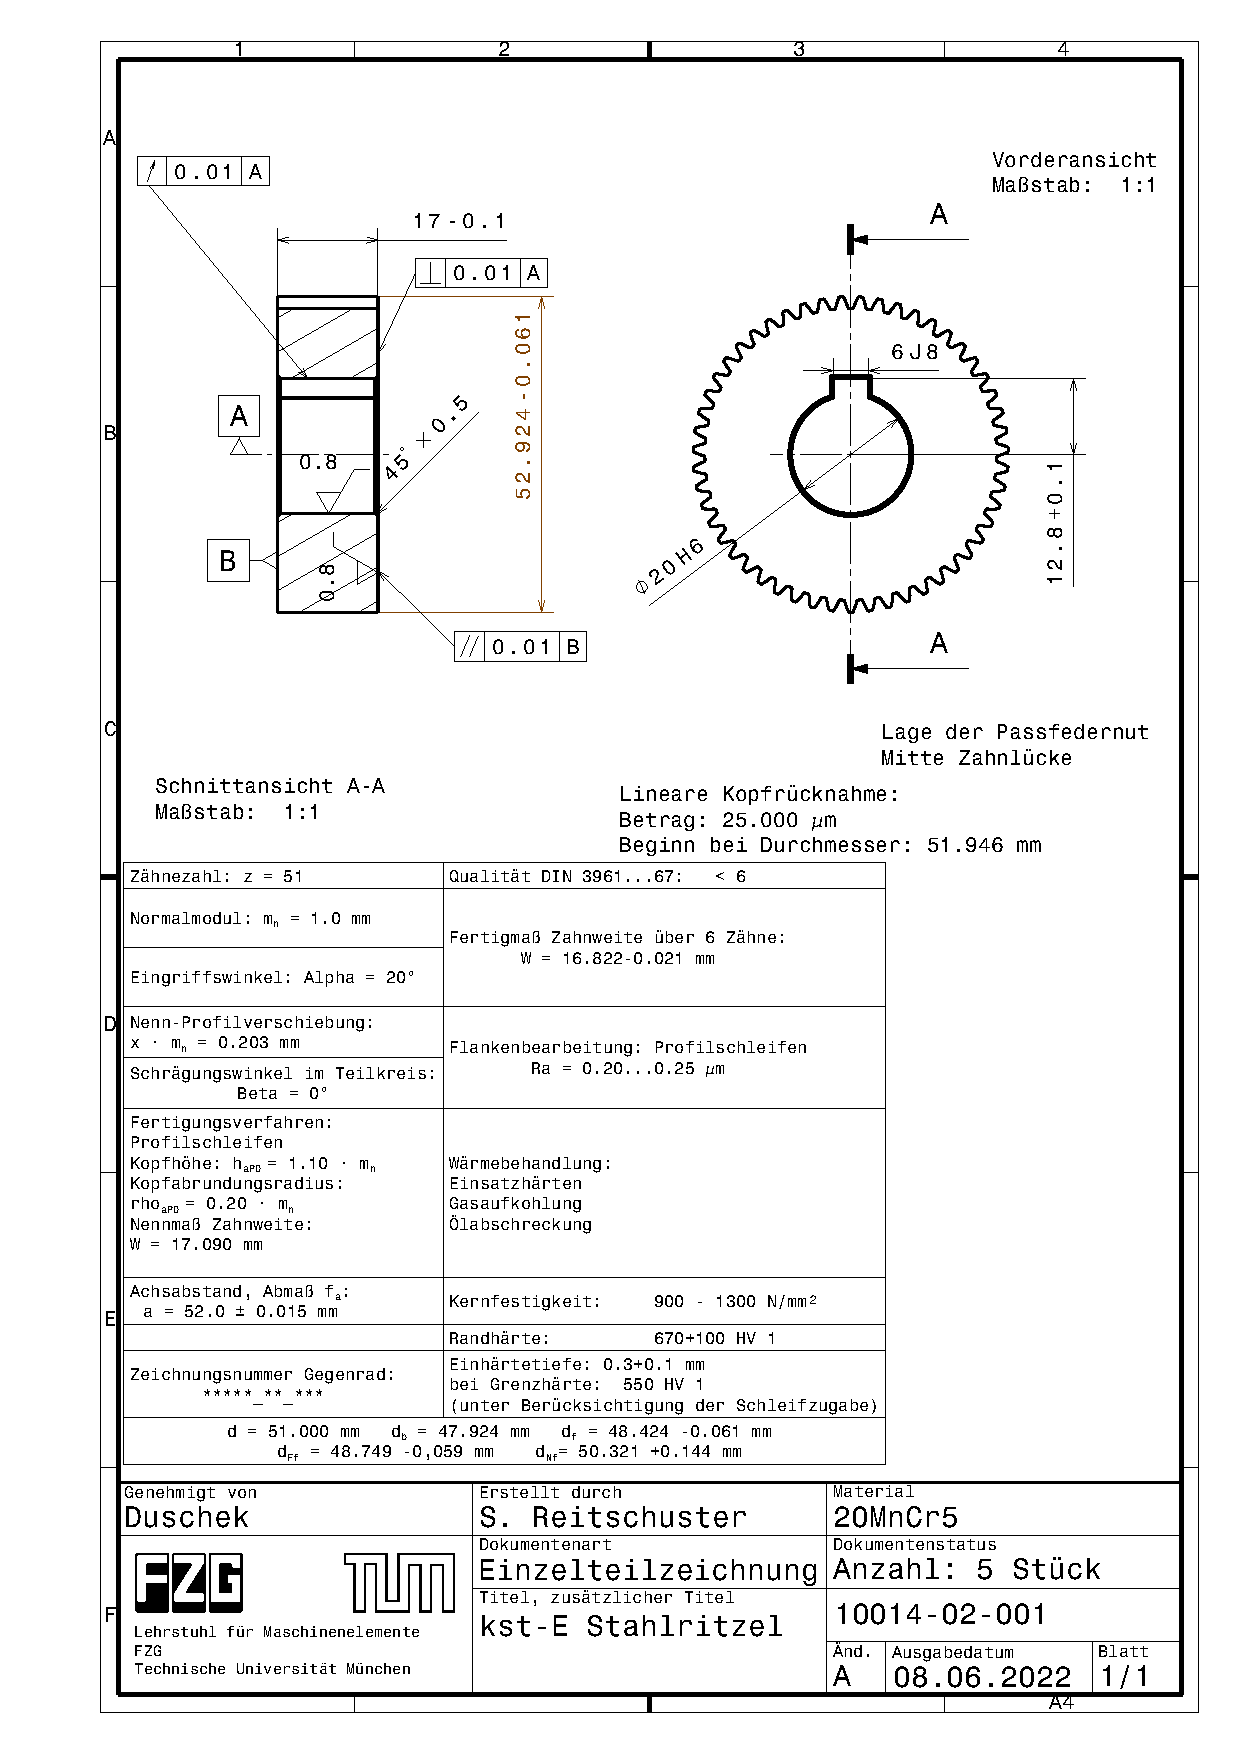
\includepdf[pages=1, scale=0.78, offset=0 -4mm, pagecommand={\thispagestyle{plain}}]{anhang/zeichnung_ritzel_2022.pdf}
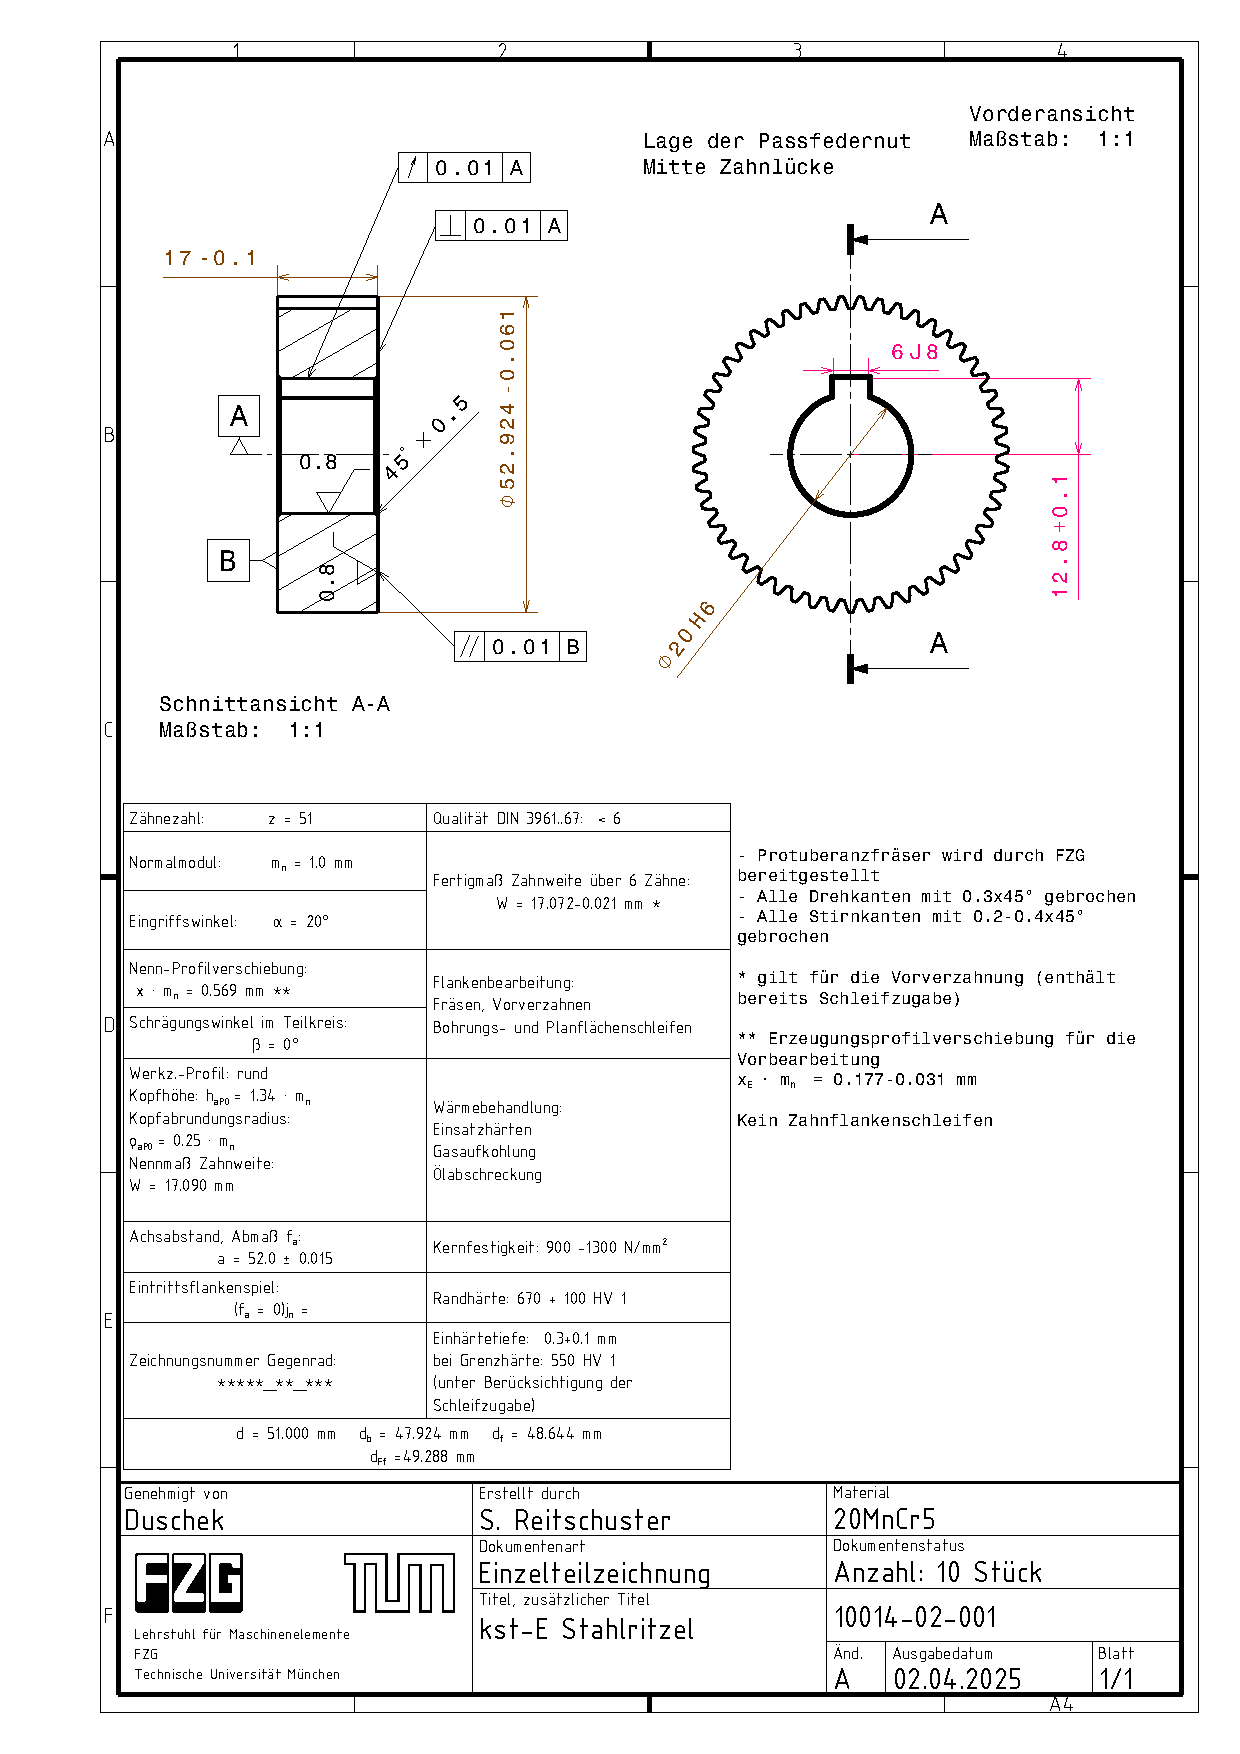
\includepdf[pages=1, scale=0.78, offset=0 -4mm, pagecommand={\thispagestyle{plain}}]{anhang/zeichnung_ritzel_2025.pdf}
